\documentclass[]{article}
\newcommand{\FileDepth}{../../..}
\usepackage[letterpaper, landscape, margin=0.5cm]{geometry}
\usepackage[T1]{fontenc}
\usepackage{textcomp}%Not strictly necessary, but gives \textmu command for "micro."
\usepackage{fancyhdr}
\usepackage{amsmath}
\usepackage{amssymb}
\usepackage{graphicx}
\usepackage{xcolor}
\usepackage{tikz}
\usetikzlibrary{calc}
\usepackage[shortlabels]{enumitem}
\usepackage{multicol}
\usepackage{vwcol}
\usepackage{hyperref}
\usepackage{wrapfig}
%opening
\newcommand{\SecType}{L}
\newcommand{\Week}{24}
\title{PH 211 Lecture \Week}
\author{Benjamin Bauml}
\date{Summer 2024}

\newcommand{\Purpose}{4}
\newcommand{\DefOnly}{0}

\input{\FileDepth/Formats/Assignment20240614.tex}
\usepackage[absolute]{textpos}
% This package relies on Assignment Format 2024-06-14 or later to work. It is recommended that the Purpose and DefOnly commands be given as such:
%\newcommand{\Purpose}{4}
%\newcommand{\DefOnly}{0}
% Activities need to be entered outside of the TeacherMargin and PresentSpace environments, otherwise they will be defined only locally. They can even go in the preamble.
\newenvironment{TeacherMargin}{\begin{textblock*}{10.8cm}(0.5cm,0.5cm)
\small}{\end{textblock*}
\hspace{0.1cm}}
\newenvironment{PresentSpace}{\begin{textblock*}{0.3cm}(26.85cm,9.35cm)
--
\end{textblock*}
\begin{textblock*}{15.6cm}(11.8cm,0.5cm)
\begin{Repurpose}{1}
\Large}{\end{Repurpose}
\end{textblock*}
\hspace{0.1cm}}

\newcommand{\FBDaxes}[4][2]{
	\begin{scope}[shift={(#2)},rotate=#3]
		% x-axis
		\draw[thick,->] (-#1,0) -- (#1,0);
		\node[anchor=west] at (#1,0) {$x$};
		% y-axis
		\draw[thick,->] (0,-#1) -- (0,#1);
		\node[anchor=south] at (0,#1) {$y$};
		\coordinate (#4) at (0,0);
	\end{scope}
}
\newcommand{\FBDvectorMA}[4]{
	\begin{scope}[shift={(#1)}]
		\coordinate (#4tip) at ({#2*cos(#3)},{#2*sin(#3)});
		\draw[ultra thick,blue,->] (#1) -- (#4tip);
	\end{scope}
}
\newcommand{\FBDvectorXY}[3]{
	\begin{scope}[shift={(#1)}]
		\coordinate (#3tip) at (#2);
		\draw[ultra thick,blue,->] (0,0) -- (#3tip);
	\end{scope}
}
\newcommand{\FBDdot}[1]{
	\filldraw[black] (#1) circle (3pt);
}
\newcommand{\FBDbox}[5][1]{
	\begin{scope}[shift={(#2)},rotate=#3]
		\filldraw[color=black,fill=white,thick] ({-#1/2},{#1/2}) -- ({-#1/2},{-#1/2}) -- ({#1/2},{-#1/2}) -- ({#1/2},{#1/2}) -- cycle;
		% Left side coordinates
		\coordinate (#4ltq) at ({-#1/2},{#1/4});
		\coordinate (#4lcent) at ({-#1/2},0);
		\coordinate (#4lbq) at ({-#1/2},{-#1/4});
		% right side coordinates
		\coordinate (#4rtq) at ({#1/2},{#1/4});
		\coordinate (#4rcent) at ({#1/2},0);
		\coordinate (#4rbq) at ({#1/2},{-#1/4});
		% top coordinates
		\coordinate (#4tlq) at ({-#1/4},{#1/2});
		\coordinate (#4tcent) at (0,{#1/2});
		\coordinate (#4trq) at ({#1/4},{#1/2});
		% bottom coordinates
		\coordinate (#4blq) at ({-#1/4},{-#1/2});
		\coordinate (#4bcent) at (0,{-#1/2});
		\coordinate (#4brq) at ({#1/4},{-#1/2});
		% corners
		\coordinate (#4tl) at ({-#1/2},{#1/2});
		\coordinate (#4tr) at ({#1/2},{#1/2});
		\coordinate (#4bl) at ({-#1/2},{-#1/2});
		\coordinate (#4br) at ({#1/2},{-#1/2});
		\node at (0,0) {#5};
	\end{scope}
}
%\newcommand{\MVec}[3][0]{%Creates a momentum vector of length #3 centered at #2 and rotated #1 degrees counterclockwise.
	\begin{scope}[rotate=#1,shift={(#2)}]
		\draw[->,thick] ({-#3/2},0) -- ({#3/2},0);
	\end{scope}
}
\newcommand{\MDot}[1]{%Creates a dot at #1 to represent a zero vector.
	\filldraw (#1) circle (1pt);
}
\newcommand{\MVDRows}[2][4.5]{%Creates the rows (initial, delta, final) of a momentum vector diagram. The optional argument determines the width of the table, and defaults to a good length for three columns (two objects and the total system). The non-optional argument gives a coordinate name (not displayed) to the diagram.
	\begin{scope}
		%\draw[thick] (0,5.5) -- (0,0);
		\draw[thick] (-1,4.5) -- (#1,4.5);
		\node at (-0.5,3.75) {$\vec{p}_{i}$};
		\draw[thick] (-1,3) -- (#1,3);
		\node at (-0.5,2.25) {$\Delta\vec{p}$};
		\draw[thick] (-1,1.5) -- (#1,1.5);
		\node at (-0.5,0.75) {$\vec{p}_{f}$};
		\coordinate (#2) at (0,5);
	\end{scope}
}
\newcommand{\MVDCol}[4][0.75]{%Creates a column for an object in a momentum vector diagram. The first (non-optional) argument is the coordinate name (not displayed) of the column, while the second is the displayed column header. The first argument also names the three entries down the column. The third argument anchors the column, so it should either be the coordinate name of the MVD (for the first column) or the coordinate name of the previous column. The optional argument indicates how far the center of the column should be from the previous column's edge, and defaults to 0.75.
	\begin{scope}[shift={(#4)}]
		\node at (#1,0) {#3};
		%\draw[thick] ({#1*2},0.5) -- ({#1*2},-5);
		\draw[thick] (0,0.5) -- (0,-5);
		\coordinate (#2init) at (#1,-1.25);
		\coordinate (#2delt) at (#1,-2.75);
		\coordinate (#2fin) at (#1,-4.25);
		\coordinate (#2) at ({#1*2},0);
	\end{scope}
}

%\input{\FileDepth/Activities/Activity_One/Activity_One.tex}
%\input{\FileDepth/Activities/Activity_Two/Activity_Two.tex}

\begin{document}
\begin{TeacherMargin}

\end{TeacherMargin}
\begin{PresentSpace}
\begin{center}
	\huge Concluding Lecture (L\Week): Choosing a Model
\end{center}
\vspace{0.5cm}
\underline{Warm-Up Activity} \\
What was the topic you found most interesting in PH 211?
%\begin{multicols}{2}
\begin{enumerate}[(A)]
	\item Kinematics
	\item Forces
	\item Energy
	\item Momentum
\end{enumerate}
%\end{multicols}
\end{PresentSpace}
\newpage
\begin{TeacherMargin}

\end{TeacherMargin}
\begin{PresentSpace}
\textbf{A Model for Motion}
\begin{multicols}{2}
	Quantities
	\begin{itemize}
		\item Position: $\vec{r}$
		\item Velocity: $\vec{v}=\frac{d\vec{r}}{dt}$
		\item Acceleration: $\vec{a}=\frac{d\vec{v}}{dt}$
	\end{itemize}
	\vspace{1cm}
	Assumptions
	\begin{itemize}
		\item Use the Particle Model
	\end{itemize}
\end{multicols}
Motion Diagram
\begin{figure}[h]
	\centering
	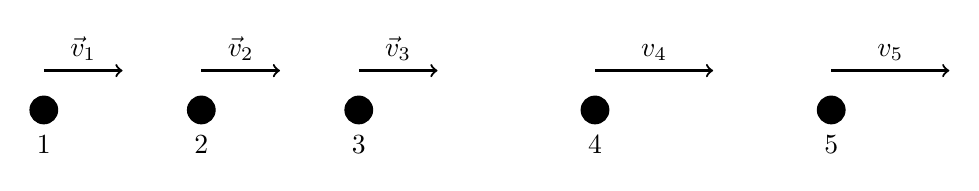
\begin{tikzpicture}
		\foreach \x in {1,2,3}
		\filldraw (2*\x,0) circle (5pt);
		\foreach \x in {1,2,3}
		\node[anchor=north] at (2*\x,-0.2) {\x};
		\foreach \x in {1,2,3}
		\draw[thick,->] (2*\x,0.5) -- (2*\x+1,0.5);
		\foreach \x in {1,2,3}
		\node[anchor=south] at (2*\x+0.5,0.5) {$\vec{v}_{\x}$};
		\begin{scope}[shift={(-3,0)}]
			\foreach \x in {4,5}
			\filldraw (3*\x,0) circle (5pt);
			\foreach \x in {4,5}
			\node[anchor=north] at (3*\x,-0.2) {\x};
			\foreach \x in {4,5}
			\draw[thick,->] (3*\x,0.5) -- (3*\x+1.5,0.5);
			\foreach \x in {4,5}
			\node[anchor=south] at (3*\x+0.75,0.5) {$v_{\x}$};
		\end{scope}
	\end{tikzpicture}
\end{figure}
\end{PresentSpace}
\newpage
\begin{TeacherMargin}

\end{TeacherMargin}
\begin{PresentSpace}
\vspace{-10pt}
\section*{A Model for Interactions}
\vspace{-10pt}
\begin{itemize}
	\item Quantities
	\begin{itemize}
		\item Mass \quad $m$ \qquad \textbf{--} Force \quad $\vec{F}$
		%\item Force \quad $\vec{F}$
	\end{itemize}
	\item Laws
	\begin{itemize}
		\item Net force is proportional to acceleration: \\
		$\vec{F}^{net}=m\vec{a}$
		\item Forces come in pairs: $\vec{F}_{AB} = -\vec{F}_{BA}$
	\end{itemize}
	\item Asssumptions
	\begin{itemize}
		\item We can treat multiple objects as a system.
		\item All forces act as if on the center of the system.
	\end{itemize}
\end{itemize}
\end{PresentSpace}
\begin{textblock*}{5cm}(22cm,1.34cm)
\Large
\begin{itemize}
	\item Diagram
\end{itemize}
\centering
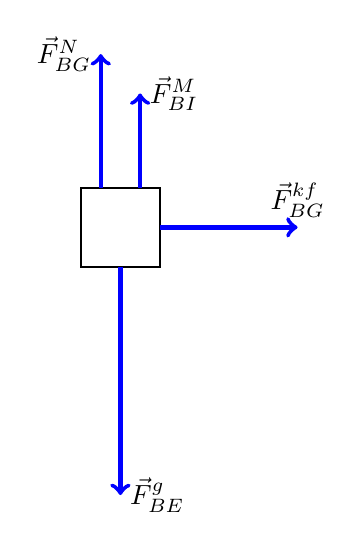
\begin{tikzpicture}
	\FBDbox{0,0}{0}{box}{}
	\FBDvectorXY{boxtrq}{0,1.2}{FM}
	\node[anchor=west] at (FMtip) {$\vec{F}^{M}_{BI}$};
	\FBDvectorXY{boxtlq}{0,1.7}{FN}
	\node[anchor=east] at (FNtip) {$\vec{F}^{N}_{BG}$};
	\FBDvectorXY{boxrcent}{1.75,0}{FKF}
	\node[anchor=south] at (FKFtip) {$\vec{F}^{kf}_{BG}$};
	\FBDvectorXY{boxbcent}{0,-2.9}{FG}
	\node[anchor=west] at (FGtip) {$\vec{F}^{g}_{BE}$};
\end{tikzpicture}
\end{textblock*}
\newpage
\begin{TeacherMargin}

\end{TeacherMargin}
\begin{PresentSpace}
\vspace{-10pt}
\section*{Types of Forces}
\vspace{-10pt}
\begin{itemize}
	\item Gravity \qquad \qquad \qquad \qquad $\vec{F}^{g}_{AB} = m_{A}\vec{g}_{B}$
	\begin{itemize}
		\item Newtonian \qquad\ $\vec{g}_{B} = G\frac{M_{B}}{r^{2}}(-\hat{r})$, $G = 6.67408\times10^{-11}\text{ N}\cdot\text{m}^{2}/\text{kg}^{2}$
		\item Near-Earth \qquad $\vec{g}_{E} = g(-\hat{y}),\ g=9.81\frac{\text{m}}{\text{s}^{2}} \approx 10\frac{\text{m}}{\text{s}^{2}}$
	\end{itemize}
	\item Normal \qquad $\vec{F}^{N}$ always $\bot$; varies in magnitude
	\item Tension \qquad $\vec{F}^{T}$ uniform (massless, inextensible rope)
	\item Spring \qquad $\vec{F}^{S}=-k(\vec{x}-\vec{x}_{eq})$
	\item Friction
	\begin{itemize}
		\item Static Friction \qquad $F^{sf}\leq\mu_{s}|\vec{F}^{N}|$
		\item Kinetic Friction \qquad $F^{kf}=\mu_{k}|\vec{F}^{N}|$
	\end{itemize}
\end{itemize}
\end{PresentSpace}
\begin{textblock*}{5cm}(22cm,6cm)
\Large
\noindent\textbf{Not Forces}
\begin{itemize}
	\normalsize
	\item Momentum
	\item Inertia
	\item Velocity
	\item Acceleration
\end{itemize}
\end{textblock*}
\newpage
\begin{TeacherMargin}

\end{TeacherMargin}
\begin{PresentSpace}
\vspace{-10pt}
\section*{A Deeper Model for Interactions}
\vspace{-10pt}
\begin{itemize}
	\item Quantities
	\begin{itemize}
		\item Energy \qquad \qquad \qquad \quad \ \ $E$
		\item Work \qquad \qquad \qquad \quad \ \ \ \ $W = \int_{r_{i}}^{r_{f}}\vec{F}\cdot d\vec{r}$
		\item Kinetic Energy \qquad \qquad $K=\frac{1}{2}mv^{2}$
		\item Potential Energy \qquad \quad \ $U=$ depends on interaction \\
		You have to tell everyone where zero $PE$ is!
		\begin{itemize}
			\item Gravity \qquad $U_{g} = mgy$
			\item Spring \qquad \ $U_{sp} = \frac{1}{2}kx^{2}$
		\end{itemize}
		\item Momentum \qquad \qquad \qquad $\vec{p}=m\vec{v}$
		\item Impulse \qquad \qquad \quad \quad \ \ $\vec{J}_{net}=\int_{t_{i}}^{t_{f}}\vec{F}^{net}dt$
	\end{itemize}
	\item Laws
	\begin{itemize}
		\item Work-energy theorem \qquad $W_{\text{net,ext}} = \Delta E_{\text{total}}$
		\item Impulse-momentum theorem \qquad $\vec{J}_{net} = \Delta\vec{p}$
	\end{itemize}
\end{itemize}
\end{PresentSpace}
\newpage
\begin{TeacherMargin}

\end{TeacherMargin}
\begin{PresentSpace}
\vspace{-10pt}
\section*{Putting the Pieces Together}
\vspace{-10pt}
\begin{itemize}
	\item How do we use problems we've already solved to help us solve new ones?
	\item For each scenario, which model(s) would you use, and why?
	\begin{itemize}
		\item Kinematics (motion, projectiles)
		\item Forces (friction, springs, multiple objects)
		\item Energy (work, power, potential energy, systems)
		\item Momentum (impulse, systems)
	\end{itemize}
\end{itemize}
\end{PresentSpace}
\newpage
\begin{TeacherMargin}

\end{TeacherMargin}
\begin{PresentSpace}
\vspace{-10pt}
\section*{L\Week-1: Choosing a Model -- Dart}
\vspace{-5pt}
A dart is thrown horizontally at a speed of 10 m/s directly at the bullseye of a dartboard 2.4 meters away from the thrower. \\

\noindent Where does the dart strike the board?
\end{PresentSpace}
\newpage
\begin{TeacherMargin}

\end{TeacherMargin}
\begin{PresentSpace}
\vspace{-10pt}
\section*{L\Week-2: Choosing a Model -- The Ramp}
\vspace{-5pt}
A stunt cyclist builds a ramp that will allow the cyclist to coast down the ramp and jump over several parked cars, as shown below. To test the ramp, the cyclist starts from rest at the top of the ramp, coasts down to the bottom, jumps over six cars, and lands on a second ramp. \\

\noindent Goal: Derive an expression for $X_{0}$.
\begin{center}
	\small
	Problem Credit: College Board \textcopyright 2021
\end{center}
\end{PresentSpace}
\newpage
\begin{TeacherMargin}
\begin{center}
	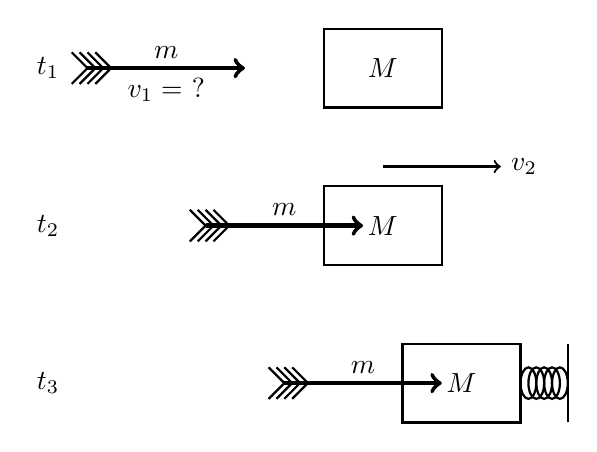
\begin{tikzpicture}
		\node at (-3.5,0) {$t_{1}$};
		\begin{scope}[shift={(-3,0)}]
			\draw[thick] (-0.2,0.2) -- (0,0) -- (-0.2,-0.2);
			\draw[thick] (-0.1,0.2) -- (0.1,0) -- (-0.1,-0.2);
			\draw[thick] (0,0.2) -- (0.2,0) -- (0,-0.2);
			\draw[thick] (0.1,0.2) -- (0.3,0) -- (0.1,-0.2);
			\draw[ultra thick,->] (0,0) -- (2,0);
			\node[anchor=south] at (1,0) {$m$};
			\node[anchor=north] at (1,0) {$v_{1}=\ ?$};
		\end{scope}
		\begin{scope}
			\draw[thick] (0,-0.5) rectangle (1.5,0.5);
			\node at (0.75,0) {$M$};
			%\draw[thick,->] (0.75,0.75) -- (2.25,0.75) node[anchor=west] {$v_{2}$};
		\end{scope}
		\begin{scope}[shift={(0,-2)}]
			\node at (-3.5,0) {$t_{2}$};
			\begin{scope}[shift={(-1.5,0)}]
				\draw[thick] (-0.2,0.2) -- (0,0) -- (-0.2,-0.2);
				\draw[thick] (-0.1,0.2) -- (0.1,0) -- (-0.1,-0.2);
				\draw[thick] (0,0.2) -- (0.2,0) -- (0,-0.2);
				\draw[thick] (0.1,0.2) -- (0.3,0) -- (0.1,-0.2);
				\draw[ultra thick,->] (0,0) -- (2,0);
				\node[anchor=south] at (1,0) {$m$};
				%\node[anchor=north] at (1,0) {$v_{1}=\ ?$};
			\end{scope}
			\begin{scope}
				\draw[thick] (0,-0.5) rectangle (1.5,0.5);
				\node at (0.75,0) {$M$};
				\draw[thick,->] (0.75,0.75) -- (2.25,0.75) node[anchor=west] {$v_{2}$};
			\end{scope}
		\end{scope}
		\begin{scope}[shift={(0,-4)}]
		\node at (-3.5,0) {$t_{3}$};
			\begin{scope}[shift={(-0.5,0)}]
				\draw[thick] (-0.2,0.2) -- (0,0) -- (-0.2,-0.2);
				\draw[thick] (-0.1,0.2) -- (0.1,0) -- (-0.1,-0.2);
				\draw[thick] (0,0.2) -- (0.2,0) -- (0,-0.2);
				\draw[thick] (0.1,0.2) -- (0.3,0) -- (0.1,-0.2);
				\draw[ultra thick,->] (0,0) -- (2,0);
				\node[anchor=south] at (1,0) {$m$};
				%\node[anchor=north] at (1,0) {$v_{1}=\ ?$};
			\end{scope}
			\begin{scope}[shift={(1,0)}]
				\draw[thick] (0,-0.5) rectangle (1.5,0.5);
				\node at (0.75,0) {$M$};
				%\draw[thick,->] (0.75,0.75) -- (2.25,0.75) node[anchor=west] {$v_{2}$};
			\end{scope}
			\foreach \s in {0,1,2,3,4}
				\draw[thick] ({0.1*\s+2.6},0) circle (0.1 and 0.2);
			\draw[thick] (3.1,-0.5) -- (3.1,0.5);
		\end{scope}
	\end{tikzpicture}
\end{center}
\end{TeacherMargin}
\begin{PresentSpace}
\vspace{-10pt}
\section*{L\Week-3: Choosing a Model -- Arrow}
\vspace{-5pt}
You fire a 0.05 kg arrow at an unknown speed. It embeds in a 0.35 kg block that slides on a frictionless surface until it compresses a spring of spring constant $k=4000$ N/m a distance of 0.10 m. \\

\noindent What was the speed at which the arrow was fired?
\vspace{3.5cm}
\begin{center}
	\small
	Problem Credit: Etkina College Physics
\end{center}
\end{PresentSpace}
\newpage
\begin{TeacherMargin}

\end{TeacherMargin}
\begin{PresentSpace}
\vspace{-10pt}
\section*{L\Week-4: Choosing a Model -- Force}
\vspace{-5pt}
The plot below shows the net force applied in the $x$-direction to a 2 kg particle moving parallel to the $x$-axis. The velocity of the particle at $x=0$ is $+6$ m/s in the $x$-direction. \\

\noindent Find the particle's speed at $x=4$ m.
\begin{center}
	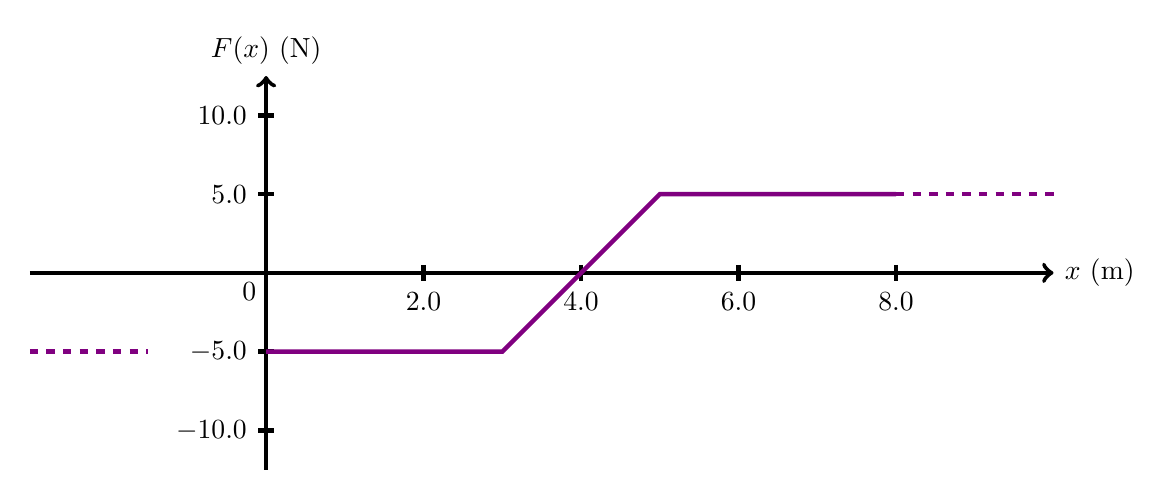
\begin{tikzpicture}
		\node[anchor=north east] at (0,0) {0};
		\draw[ultra thick,->] (-3,0) -- (10,0) node [anchor=west] {$x$ (m)};
		\foreach \x in {2.0,4.0,6.0,8.0}
			\draw[ultra thick] (\x,0.1) -- (\x,-0.1) node[anchor=north] {$\x$};
		\draw[ultra thick,->] (0,-2.5) -- (0,2.5) node [anchor=south] {$F(x)$ (N)};
		\foreach \y in {-10.0,-5.0,5.0,10.0}
			\draw[ultra thick] (0.1,\y/5) -- (-0.1,\y/5) node[anchor=east] {$\y$};
		\draw[ultra thick,violet] (0,-1) -- (3,-1) -- (5,1) -- (8,1);
		\draw[ultra thick,dashed,violet] (-3,-1) -- (-1.5,-1);
		\draw[ultra thick,dashed,violet] (8,1) -- (10,1);
	\end{tikzpicture} \\
	\small
	Problem Credit: OpenStax University Physics
\end{center}
\end{PresentSpace}
\newpage
\begin{TeacherMargin}
	
\end{TeacherMargin}
\begin{PresentSpace}
\section*{Main Ideas}
\begin{itemize}
	\item This concludes the course.
	\item We've tried to introduce you to how a physicist looks at the universe.
	\item I hope you feel more capable than at the beginning of the term.
	\item Congratulate yourself for working so hard!
\end{itemize}
\end{PresentSpace}
\end{document}